\chapter{Dynamic Modeling}
\section{Introduction and Objectives}
The central technical contribution of this work, within the broader context of the exoskeleton project, consists in the development of a physics-based digital twin capable of \textbf{reproducing the dynamic behavior} of the mechanical transmission in real time within a ROS 2 environment. This chapter addresses the mathematical modeling of the mechanism and the software implementation of its reduced dynamic representation.

The exoskeleton mechanism under consideration is characterized by a multibody structure composed of several rigid links connected through revolute and prismatic joints. The transmission includes multiple closed kinematic loops and nonlinear geometric constraints, yet it is driven by a single actuated joint located at the crank. This structural characteristic plays a crucial role in the modeling strategy adopted in this work.

A straightforward formulation of the complete system dynamics would lead to a constrained multibody problem described by differential-algebraic equations. Such an approach, although formally rigorous, would require the real-time solution of a high-dimensional system subject to algebraic constraints. In a distributed ROS 2 architecture, where the dynamic node must operate at high frequency and interact with other modules, this computational burden would compromise numerical robustness and real-time determinism.

To overcome this limitation, a \textbf{reduction strategy} was developed. The key idea is to exploit the intrinsic single-degree-of-freedom nature of the mechanism and to reformulate the constrained multibody dynamics in terms of a single generalized coordinate, namely the crank angle. By projecting the full dynamics onto this reduced coordinate, it becomes possible to derive a scalar nonlinear dynamic equation that preserves the essential physical effects of the original system while drastically reducing computational complexity.

The digital twin developed in this work is therefore designed to reproduce the nonlinear dynamic response of the mechanism under an applied motor torque, taking into account inertial effects, gravitational contributions, friction phenomena, external interaction forces and, in the extended model, passive biomechanical torques associated with the hand joints. At the same time, the implementation must guarantee numerical stability, robustness against kinematic singularities and compatibility with the ROS 2 communication infrastructure.

Two dynamic nodes were implemented following the same theoretical framework. The first describes the exoskeleton transmission alone, while the second extends the model to include the hand subsystem and its passive elastic behavior. The mathematical structure remains identical in both cases; the extended model introduces additional generalized coordinates and passive torque contributions but preserves the same reduction philosophy.

The remainder of this chapter first introduces the complete constrained multibody formulation of the system, then derives the reduced-order dynamic model, and finally discusses its numerical implementation within the ROS 2 environment.

\section{Full Multibody Model of the Exoskeleton}
\subsection{URDF-Based Rigid-Body Representation}
The mechanical structure of the exoskeleton is described using the Unified Robot Description Format (URDF), which provides a standardized way to encode the kinematic and inertial properties of robotic systems. Two URDF models are considered in this work: one representing the transmission mechanism only and a second, extended version including the finger phalanges and hand components. Both models share the same structural principles and differ only in the number of links and joints.

Each URDF file defines a set of rigid links, their mass properties and inertia tensors, as well as the joints connecting them. The inertial parameters are assumed to be constant and lumped at the link level. All bodies are treated as perfectly rigid, and all joints are modeled as ideal kinematic pairs without backlash, compliance or structural flexibility. These assumptions are consistent with the objective of developing a real-time dynamic twin focused on the dominant mechanical behavior of the system.

The URDF description is imported into the Pinocchio rigid-body dynamics library, which automatically constructs the underlying multibody model. This model provides access to forward kinematics, frame placements, Jacobians, the joint-space inertia matrix, and the nonlinear terms including Coriolis and gravitational effects. The availability of these quantities is fundamental for both the dynamic formulation and the reduction procedure described later.

Although the URDF representation is inherently tree-structured, the exoskeleton mechanism contains closed kinematic loops that cannot be directly expressed within a pure tree topology. To address this issue, additional geometric constraints are enforced at runtime. These constraints are defined through pairs of frames whose spatial coincidence must be maintained during motion. Consequently, the URDF model serves as the underlying open-chain representation, while the loop closure conditions are imposed numerically during simulation.

\subsection{Constrained Multibody Dynamic Formulation}
Let $\textbf{q} \in \textbf{R}^n$ denote the vector of generalized coordinates associated with the URDF model. In the absence of constraints, the rigid-body dynamics of the system can be expressed in standard form as

\begin{equation}
\textbf{M}(\textbf{q})\ddot{\textbf{q}} + \textbf{h}(\textbf{q},\dot{\textbf{q}}) = \tau
\end{equation}

where $\textbf{M}(\textbf{q})$ is the joint-space inertia matrix, $\textbf{h}(\textbf{q},\dot{\textbf{q}})$ represents the nonlinear Coriolis, centrifugal and gravitational terms, and $\tau$ is the vector of generalized forces applied at the joints. 

However, due to the presence of closed loops, the generalized coordinates are not independent. The mechanism is subject to holonomic constraints that can be written as

\begin{equation}
\Phi(\textbf{q}) = \textbf{0}
\end{equation}

where $\Phi \in \textbf{R}^m$ is a vector-valued function representing the geometric constraints. The number of constraints $m$ corresponds to the number of independent loop closure conditions.

To incorporate these constraints into the dynamic formulation, Lagrange multipliers $\lambda \in \textbf{R}^m$ are introduced, leading to the constrained dynamic model:

\begin{equation}
\textbf{M}(\textbf{q})\ddot{\textbf{q}} + \textbf{h}(\textbf{q},\dot{\textbf{q}}) = \tau + \textbf{J}^T(\textbf{q})\lambda
\end{equation}

where the constraint Jacobian is defined as

\begin{equation}
\textbf{J}(\textbf{q}) = \frac{\partial \Phi(\textbf{q})}{\partial \textbf{q}}
\end{equation}

The complete system is therefore composed of second-order differential equations coupled with algebraic constraint equations. This structure results in a differential-algebraic system whose direct real-time solution would require dedicated numerical techniques and constraint stabilization methods. Such an approach would significantly increase computational cost and introduce potential numerical stiffness issues.

Nevertheless, the mechanical architecture of the exoskeleton transmission possesses a fundamental property: despite the apparent complexity of the multibody structure, the system has \textbf{only one independent degree of freedom}. The remaining coordinates are entirely determined by the closure constraints once the crank angle is specified. This observation enables a systematic reduction of the full constrained model to a scalar nonlinear dynamic equation, as will be derived in the following section.

\section{Reduction to a 1-DoF Dynamic Model}
\subsection{Selection of the Independent Generalized Coordinate}
As discussed in the previous section, the complete multibody system described by the URDF model is subject to holonomic closure constraints. Although the generalized coordinate vector $\textbf{q} \in \textbf{R}^n$ formally contains multiple joint variables, the mechanical architecture of the transmission ensures that the mechanism possesses only one independent degree of freedom.

From a physical standpoint, the configuration of the entire mechanism is uniquely determined by the rotation of the crank joint. Once the crank angle is fixed, the positions of all other joints are geometrically constrained by the loop closure conditions. This structural property motivates the choice of the crank angle as the independent generalized coordinate of the reduced model.

Let the scalar variable
\begin{equation}
\theta := \textbf{q}_{crank}
\end{equation}

represent the angular position of the actuated crank joint. All other generalized coordinates can then be interpreted as implicit functions of $\theta$, determined by the nonlinear constraint equations:

\begin{equation}
\Phi(\textbf{q}) = \textbf{0}
\end{equation}

Consequently, the full coordinate vector may be expressed as

\begin{equation}
\textbf{q} = \textbf{q}(\theta)
\end{equation}

with the understanding that this mapping is defined implicitly through the closure conditions.

This choice enables the reformulation of the entire system dynamics in terms of a single scalar variable, significantly reducing computational complexity while preserving physical consistency.


\subsection{Velocity-Level Constraint Reduction}
\textbf{The reduction procedure can be derived formally by differentiating the holonomic constraints with respect to time.} Starting from the constraint equations

\begin{equation}
\Phi(\textbf{q}(\theta)) = \textit{p}_A - \textit{p}_B = \textbf{0}
\end{equation}

where $\textit{p}_A$ and $\textit{p}_B$ are the positions of the coupled auxiliary frames, the first time derivative yields the velocity-level constraints:

\begin{equation}
(\textbf{J}_A(\textbf{q}) - \textbf{J}_B(\textbf{q}))\dot{\textbf{q}} = \textbf{J}_c(\textbf{q})\dot{\textbf{q}} = \textbf{0}
\end{equation}

where $\textbf{J}_c(\textbf{q})$ is the \textbf{constraint Jacobian}. 

This equation indicates that the velocity vector $\dot{\textbf{q}}$ must lie in the null space of the constraint Jacobian. Since the system has only one degree of freedom, the null space is one-dimensional and can be parameterized by the scalar variable $\dot{\theta}$:
\begin{equation}
\dot{\textbf{q}} = \textbf{B}(\textbf{q})\dot{\theta}
\end{equation}  

where $\textbf{B}(\textbf{q}) \in \textbf{R}^n$ represents the vector of generalized velocity coefficients and corresponds to the derivative of the full coordinate vector with respect to the crank angle:

\begin{equation}
\textbf{B}(\textbf{q}) = \frac{\partial \textbf{q}}{\partial \theta}
\end{equation}  

In practice, this vector is computed numerically by solving a linear system derived from the constraint Jacobian. The crank component is fixed to unity, and the remaining components are obtained by solving a least-squares problem that enforces the velocity-level constraints. This procedure guarantees that the reconstructed velocity vector remains consistent with the geometric closure conditions.

The same projection framework can be extended to accelerations by differentiating once more, leading to

\begin{equation}
\ddot{\textbf{q}} = \textbf{B}(\textbf{q})\ddot{\theta} + \dot{\textbf{B}}(\textbf{q})\dot{\theta}
\end{equation}

\subsection{Projection of the Full Dynamics}
With the velocity and acceleration expressed in terms of the scalar variable $\theta$, the full multibody dynamics can be projected onto the reduced coordinate. 

Starting from the constrained dynamic equation

\begin{equation}
\textbf{M}(\textbf{q})\ddot{\textbf{q}} +
\textbf{C}(\textbf{q},\dot{\textbf{q}})\dot{\textbf{q}} +
\textbf{g}(\textbf{q}) 
= \tau + \textbf{J}^T(\textbf{q})\lambda
\end{equation}  

The key idea of the reduction is to eliminate the unknown constraint forces $\lambda$ by projecting the dynamics onto the null space of the constraint Jacobian. This is achieved by premultiplying both sides of the equation by $\textbf{B}^T(\textbf{q})$, which yields:

\begin{equation}
\textbf{B}^T(\textbf{q})\textbf{M}(\textbf{q})\ddot{\textbf{q}} +
\textbf{B}^T(\textbf{q})\textbf{C}(\textbf{q},\dot{\textbf{q}})\dot{\textbf{q}} +
\textbf{B}^T(\textbf{q})\textbf{g}(\textbf{q})
= \textbf{B}^T(\textbf{q})\tau  
\end{equation}

Doing so, the contribution of the constraint forces is eliminated since 

\begin{equation}
\textbf{B}^T(\textbf{q})\textbf{J}^T(\textbf{q})\lambda =
(\textbf{J}(\textbf{q})\textbf{B}(\textbf{q}))^T\lambda = 0
\end{equation}

and $\textbf{J}(\textbf{q})\textbf{B}(\textbf{q})$ is identically zero by construction.

Substituting the expressions for $\dot{\textbf{q}}$ and $\ddot{\textbf{q}}$ in terms of $\theta$ (equations \textbf{3.10} and \textbf{3.12}) in equation \textbf{3.14}, the reduced dynamic equation can be written in the standard form, ignoring the explicit dependence on $\textbf{q}$ and $\dot{\textbf{q}}$ for brevity:

\begin{equation}
\textbf{B}^T\textbf{M}(\textbf{B}\ddot{\theta} + \dot{\textbf{B}}\dot{\theta}) + \textbf{B}^T\textbf{h} = \textbf{B}^T\tau
\end{equation}

Doing the matrix multiplication, the final form of the reduced dynamic equation is obtained:

\begin{equation}
\textbf{B}^T\textbf{M}\textbf{B}\ddot{\theta} + \textbf{B}^T\textbf{M}\dot{\textbf{B}}\dot{\theta} + \textbf{B}^T\textbf{h} = \textbf{B}^T\tau
\end{equation}

The first term

\begin{equation*}
    \textbf{B}^T\textbf{M}\textbf{B}\ddot{\theta}
\end{equation*}

represents the \textbf{effective inertia of the entire multibody system projected onto the crank coordinate}. The scalar quantity

\begin{equation}
I_{eff}(\theta) = \textbf{B}^T\textbf{M}(\textbf{q})\textbf{B}
\end{equation}

can be interpreted as the equivalent inertia seen at the motor shaft. Although the full inertia matrix $\textbf{M}(\textbf{q})$ depends on all generalized coordinates, the projection through $\textbf{B}$ condenses the coupled inertial effects of all links into a single scalar function of the crank angle. This term captures the nonlinear redistribution of mass throughout the mechanism as the configuration evolves.

The second term

\begin{equation*}
    \textbf{B}^T\textbf{M}\dot{\textbf{B}}\dot{\theta} 
\end{equation*}

originates from the time variation of the projection vector $\textbf{B}(\textbf{q})$. Physically, it accounts for geometric acceleration effects associated with the curvature of the constraint manifold. In practice, this contribution behaves as a velocity-dependent inertial correction term. 

The third term
\begin{equation*}
    \textbf{B}^T\textbf{h}(\textbf{q},\dot{\textbf{q}}) 
\end{equation*}

contains the projection of Coriolis, centrifugal, and gravitational contributions onto the reduced coordinate. In the implementation, these effects are computed directly using the rigid-body dynamics algorithms provided by Pinocchio and subsequently projected onto the crank direction.

The right-hand side term
\begin{equation*}
    \textbf{B}^T\tau
\end{equation*}

represents the generalized torque projected onto the admissible motion direction. Since only the crank joint is actuated, the torque vector $\tau$ contains a single nonzero component equal to the motor torque $\tau_{m}$. 

Additional contributions such as friction, passive elastic torques and externally applied wrenches are incorporated before projection.

The final reduced dynamic equation implemented in the digital twin can be expressed as

\begin{equation}
I_{eff}(\theta)\ddot{\theta} = \tau_{m} - \tau_{fric} - \tau_{ext} - \tau_{pass} 
\end{equation}

where $\tau_{fric}$ represents the total friction torque, $\tau_{ext}$ accounts for external interaction forces, and $\tau_{pass}$ includes passive biomechanical torques in the extended model. Each of these contributions is computed based on the current state of the system and projected onto the crank coordinate using the same reduction framework.

\section{Numerical Implementation of the Reduced Dynamic Model}
The reduced-order formulation derived in \textbf{Equation 3.19} leads to a scalar nonlinear equation in the crank coordinate $\theta$. In the proposed Digital Twin, this equation is evaluated numerically at runtime, following the same computational blocks implemented in the ROS 2 dynamic node. The objective is to guarantee (i) consistency with the URDF-based multibody model, (ii) compatibility with the numerical loop-closure enforcement, and (iii) deterministic execution at the node update rate.

At each simulation step, the node computes a kinematically consistent configuration $\textbf{q}(\theta)$, reconstructs the motion direction $\textbf{B}(\textbf{q})$, evaluates the full inertia matrix $\textbf{M}(\textbf{q})$ and nonlinear terms $\textbf{h}(\textbf{q},\dot{\textbf{q}})$ using Pinocchio, and integrates the scalar dynamics forward in time.

\subsection{Step-by-Step Execution Pipeline}
Let ($\theta$, $\dot{\theta}$) denote the scalar state propagated by the reduced model. The node executes the following pipeline at each time step $\Delta t$:

\begin{enumerate}
    \item \textbf{Loop closure at the current crank angle}: Given the current value of $\theta$, the node solves the nonlinear loop closure problem to find a consistent configuration $\textbf{q}(\theta)$ that satisfies the geometric constraints. This is achieved using a numerical solver that minimizes the constraint violation, starting from the previous configuration as an initial guess. The result is a kinematically valid state of the full multibody system corresponding to the specified crank angle.
    
    \item \textbf{Compute the projection direction $\textbf{B}(\textbf{q})$}: Using the constraint Jacobian at the current configuration, the node computes the projection vector $\textbf{B}(\textbf{q})$ that defines the admissible velocity direction consistent with the closure constraints. This involves solving a linear system derived from the velocity-level constraints, ensuring that $\textbf{B}$ is properly normalized.
    
    \item \textbf{Approximate the time derivative $\dot{\textbf{B}}$}: The time derivative of the projection vector is approximated using a \textbf{finite difference} scheme based on the current and previous values of $\textbf{B}$. This approximation is necessary to evaluate the geometric acceleration term in the reduced dynamics.
    
    \item \textbf{Build generalized velocities and accelerations} through the reduced mappings: 
    
    \begin{equation*}
        \dot{\textbf{q}} = \textbf{B}(\textbf{q})\dot{\theta}, \quad \ddot{\textbf{q}} = \textbf{B}(\textbf{q})\ddot{\theta} + \dot{\textbf{B}}(\textbf{q})\dot{\theta}
    \end{equation*}

    \item \textbf{Evaluate the full dynamics}: The node computes the inertia matrix $\textbf{M}(\textbf{q})$ and nonlinear terms $\textbf{h}(\textbf{q},\dot{\textbf{q}})$ using Pinocchio's dynamics algorithms. These quantities are then projected onto the crank coordinate using the previously computed $\textbf{B}$ to obtain the effective inertia, Coriolis, centrifugal and gravitational contributions in the reduced model.
    
    \item \textbf{Compute and project additional torque contributions} such as friction, external forces and passive biomechanical effects. Each of these contributions is evaluated based on the current state and projected onto the crank coordinate using the same reduction framework.
    
    \item \textbf{Solve the scalar dynamics for $\ddot{\theta}$} using the projected quantities.
    
    \item \textbf{Integrate $(\theta, \dot{\theta})$} forward in time using a numerical integration scheme to obtain the updated state for the next iteration.
\end{enumerate}

This structure mirrors the analytical reduction, but avoids solving a constrained differential-algebraic system online.

\subsection{Computation of the Admissible Motion Direction}
Once a kinematically consistent configuration $\textbf{q}$ is available from the loop closure step seen in Chapter 2, the reduced dynamics requires the evaluation of the projection vector $\textbf{B}(\textbf{q})$, which represents the unique admissible motion direction of the mechanism.

It was already shown in Equation \textbf{3.9} that the velocity-level constraints can be expressed as

\begin{equation*}
(\textbf{J}_A(\textbf{q}) - \textbf{J}_B(\textbf{q}))\dot{\textbf{q}} = \textbf{A}(\textbf{q})\dot{\textbf{q}} = \textbf{0}
\end{equation*}

where $\textbf{A}(\textbf{q})$ is the stacked Jacobian of the loop-closure constraints, obtained by concatenating the Jacobians of the coupled auxiliary frames. 

Substituting the velocity mapping gives

\begin{equation*}
\textbf{A}(\textbf{q})\textbf{B}(\textbf{q}) = \textbf{0}
\end{equation*}

The problem therefore reduces to computing a non-trivial vector $\textbf{B}(\textbf{q})$ lying in the null space of $\textbf{A}(\textbf{q})$, while enforcing that the crank joint remains the independent coordinate.

\subsubsection*{Construction of the Constraint Matrix A(q)}
The matrix $\textbf{A}(\textbf{q})$ is constructed by evaluating the Jacobians of the coupled auxiliary frames at the current configuration. Each loop closure constraint corresponds to a pair of frames whose spatial coincidence must be maintained. The Jacobian of each frame is computed using Pinocchio's kinematics algorithms, and the difference between the Jacobians of the two frames in each pair is stacked to form the complete constraint matrix.

For each auxiliary frame pair $(\textit{p}_A, \textit{p}_B)$, the translational Jacobians are computed in world-aligned representation:

\begin{minted}{python}

    for ida, idb in self.closure_frame_pairs:
            JA = pin.computeFrameJacobian(self.model, self.data, q, ida, pin.ReferenceFrame.LOCAL_WORLD_ALIGNED)[:3, :]
            JB = pin.computeFrameJacobian(self.model, self.data, q, idb, pin.ReferenceFrame.LOCAL_WORLD_ALIGNED)[:3, :]
            A_blocks.append(JA - JB)

\end{minted}

The resulting blocks are then concatenated to form the full constraint matrix $\textbf{A}(\textbf{q})$.

\begin{minted}{python}
    A = np.vstack(A_blocks)
\end{minted}

\subsubsection*{Construction of the Projection Vector B(q)}
It was already stated that the projection vector $\textbf{B}(\textbf{q})$ must satisfy the null space condition $\textbf{A}(\textbf{q})\textbf{B}(\textbf{q}) = \textbf{0}$, but this condition alone is not sufficient to uniquely determine $\textbf{B}$ since any scalar multiple of a null space vector is also a solution. 

To obtain a unique and physically consistent mapping, the implementation enforces $\theta$ as the independent coordinate.

In the multibody state vector \textbf{q}, the crank joint variable is exactly $\theta$. Therefore, by definition:

\begin{equation*}
    q_{\theta} = \theta 
\quad \Rightarrow \quad
    \frac{\partial q_{\theta}}{\partial \theta} = 1
\end{equation*}

This is implemented by imposing:

\begin{equation*}
    B_{\theta} = 1
\end{equation*}

\begin{minted}{python}

    B = np.zeros(self.nv)
    B[self.idx_theta] = 1.0

\end{minted}

which fixes the otherwise arbitrary scale of the null-space solution and guarantees that $\dot{\theta}$ coincides with the actual crank joint velocity component extracted from $\dot{\textbf{q}}$.

To impose this constraint constructively, the vector $\textbf{B}$ is partitioned into the crank component and the remaining components:

\begin{equation*}
    \textbf{B}(\textbf{q}) = \textbf{e}_{\theta} + \textbf{x}
\end{equation*}

where $\textbf{e}_{\theta}$ is the standard basis vector with a unit entry at the crank index and zeros elsewhere, and $\textbf{x}$ is an unknown correction vector to be determined.

Substituting into the null space condition gives:

\begin{equation*}
    \textbf{A}(\textbf{q})(\textbf{e}_{\theta} + \textbf{x}) = 0
    \quad \Rightarrow \quad
    \textbf{A}(\textbf{q})\textbf{e}_{\theta} =  -\textbf{A}(\textbf{q})\textbf{x}
\end{equation*}

At this stage the unknowns are only the components of \textbf{x} excluding the crank index. Let $\textbf{A}_{red}(\textbf{q})$ denote the matrix obtained by removing the column of $\textbf{A}(\textbf{q})$ corresponding to the crank index, and let $\textbf{x}_{red}$ be the corresponding reduced vector of unknowns. The system can be rewritten as:

\begin{equation*}
    \textbf{A}_{red}(\textbf{q})\textbf{x}_{red} = -\textbf{A}(\textbf{q})\textbf{e}_{\theta}
\end{equation*}

Since the closure constraints are generally redundant (overdetermined), the system is solved in the least-squares sense:

\begin{equation*}
    \textbf{x}_{red} = args\min_{\textbf{x}_{red}} \|\textbf{A}_{red}(\textbf{q})\textbf{x}_{red} + \textbf{A}(\textbf{q})\textbf{e}_{\theta}\|^2
\end{equation*}

Finally, the full correction vector $\textbf{x}$ is reconstructed by inserting $\textbf{x}_{red}$ into the non-crank indices and setting $x_{\theta} = 0$, and the admissible direction is returned as:

\begin{equation*}
    \textbf{B}(\textbf{q}) = \textbf{e}_{\theta} + \textbf{x}
\end{equation*}

\begin{minted}{python}

        e_theta = np.zeros(self.nv)
        e_theta[self.idx_theta] = 1.0

        rhs = -A @ e_theta

        mask = np.ones(self.nv, dtype=bool)
        mask[self.idx_theta] = False
        A_red = A[:, mask]

        x_red, *_ = np.linalg.lstsq(A_red, rhs, rcond=None)
        x = np.zeros(self.nv)
        x[mask] = x_red

        return e_theta + x

\end{minted}

This procedure produces a vector $\textbf{B}(\textbf{q})$ that (i) preserves the crank as the unique independent coordinate ($B_{\theta} = 1$) and (ii) satisfies the closure constraints at velocity level by construction (in least-squares sense).

\subsubsection*{Numerical Approximation of $\dot{B}$}
The time derivative of the projection vector $\dot{\textbf{B}}(\textbf{q})$ is required to evaluate the geometric acceleration term in the reduced dynamics. However, since $\textbf{B}$ is computed numerically at each time step based on the current configuration, an analytical expression for its derivative is not readily available. Therefore, a finite difference approximation is used:

\begin{equation*}
    \dot{\textbf{B}}(\textbf{q}) \approx \frac{\textbf{B}(\textbf{q}) - \textbf{B}(\textbf{q}_{prev})}{\Delta t}    
\end{equation*}

where $\textbf{q}_{prev}$ is the configuration from the previous time step. This approximation is valid under the assumption of sufficiently small time steps and smooth variations of $\textbf{B}$ with respect to $\textbf{q}$.

\subsection{Evaluate the Full Dynamics}
At each simulation step, the reduced dynamic model requires the evaluation of the multibody inertial and nonlinear terms of the full system. Although the evolution of the mechanism is described by the scalar coordinate $\theta$, the quantities entering the projected equation are computed in the complete generalized coordinate space. This ensures that all inertial couplings and configuration-dependent effects of the assembled mechanism are preserved.

The rigid-body dynamics is evaluated using the Pinocchio library, which operates directly on the URDF-based multibody model. Two fundamental quantities are computed: the joint-space inertia matrix $\textbf{M}(\textbf{q})$ and the nonlinear effects vector $\textbf{h}(\textbf{q},\dot{\textbf{q}})$.

\subsubsection*{Inertia Matrix M(q)}
The inertia matrix $\textbf{M}(\textbf{q})$ is computed using the Composite Rigid Body Algorithm (CRBA) provided by Pinocchio. This algorithm efficiently computes the joint-space inertia matrix by recursively aggregating the inertial contributions of each link, taking into account the current configuration $\textbf{q}$. The resulting matrix captures the distribution of mass and inertia throughout the mechanism and its dependence on the configuration.

The evaluation is performed at the current configuration of the mechanism, ensuring that the inertia matrix reflects the instantaneous geometry of the closed transmission. Since the configuration satisfies the closure constraints, the inertial couplings are consistent with the physically assembled system rather than the open-chain abstraction of the URDF.

\begin{minted}{python}
    M = pin.crba(self.model, self.data, q)
\end{minted}

The resulting matrix is theoretically symmetric positive definite for admissible configurations. In practice, numerical asymmetries due to floating-point operations are negligible and do not affect the subsequent scalar projection.

\subsubsection*{Nonlinear Effects $h(q, \dot{q})$}
The vector $\textbf{h}(\textbf{q},\dot{\textbf{q}})$ encompasses the Coriolis, centrifugal and gravitational contributions to the dynamics. It is computed using the Recursive Newton-Euler Algorithm (RNEA) implemented in Pinocchio, which efficiently evaluates these nonlinear effects based on the current configuration and velocity of the system.

\begin{minted}{python}
    h = pin.rnea(self.model, self.data, q, dq, np.zeros(self.nv))
\end{minted}

This routine guarantees dynamic consistency between the inertia matrix and the nonlinear terms, since both are derived from the same multibody model and inertial parameters.

\subsubsection*{Dynamic Consistency of the Full Evaluation}
A crucial aspect of the Digital Twin architecture is that the multibody dynamics is \textbf{never reduced analytically before evaluation}. Instead, the full joint-space quantities $\textbf{M}(\textbf{q})$ and $\textbf{h}(\textbf{q},\dot{\textbf{q}})$ are computed online at every time step and only subsequently projected onto the reduced coordinate.

This approach preserves:
\begin{enumerate}
    \item Configuration-dependent inertial redistribution effects.
    \item Nonlinear velocity couplings arising from the closed-chain geometry.
    \item Gravitational torque variations across the full motion range.
\end{enumerate}

As a consequence, the reduced scalar equation retains the nonlinear characteristics of the original constrained multibody system while remaining computationally efficient.


\subsection{Compute Additional Torque Contributions}
In addition to the inertial and nonlinear terms obtained from the multibody dynamics, the reduced-order model incorporates a set of additional torque contributions that capture dissipative effects, external interactions, and biomechanical behavior.

These contributions are evaluated in the full generalized coordinate space and subsequently projected onto the admissible motion direction defined by  $B(q)$, ensuring consistency with the reduction framework introduced in Section 3.3.

The resulting scalar contributions directly enter the reduced dynamic equation:

\begin{equation}
    I_{\text{eff}}(\theta)\ddot{\theta} = \tau_m - \tau_{\text{fric}} - \tau_{\text{ext}} - \tau_{\text{pass}}
\end{equation}

Each term is detailed in the following.

\paragraph{Friction Torque}
Dissipative effects arising from joint friction are modeled through a combination of viscous and Coulomb components. The friction torque is expressed as:

\begin{equation}
    \tau_{\text{fric}} = b\dot{\theta} + f_c \tanh\left(\frac{\dot{\theta}}{\varepsilon}\right)
\end{equation}

where $b$ is the viscous friction coefficient and $f_c$ represents the Coulomb friction level. The hyperbolic tangent function provides a smooth approximation of the discontinuous sign function, ensuring numerical stability around zero velocity.

This formulation captures both velocity-proportional dissipation and static friction effects while avoiding non-differentiable behavior that could degrade the performance of the numerical integrator.

\paragraph{External Interaction Torque}

External forces applied to the mechanism, arising from contact with the user or the environment, are incorporated through a generalized torque contribution.

Let $f_{\text{ext}} \in \mathbb{R}^3$ denote the external force applied at a given contact point. The corresponding joint-space torque is obtained through the Jacobian transpose mapping:

\begin{equation}
    \tau_{\text{ext}}^{(q)} = J_{cp}(q)^T f_{\text{ext}}
\end{equation}

where $J_{cp(q)}$ is the Jacobian of the contact point.

The contribution is then projected onto the reduced coordinate using the admissible motion direction:

\begin{equation}
    \tau_{\text{ext}} = B(q)^T \tau_{\text{ext}}^{(q)}
\end{equation}

This procedure ensures that only the component of the external interaction consistent with the constrained motion of the mechanism contributes to the scalar dynamics.

\paragraph{Passive biomechanical torque}
In the extended model including the finger phalanges, passive biomechanical effects are introduced through a nonlinear elastic-dissipative model acting on the anatomical joints. In particular, the metacarpophalangeal and proximal interphalangeal joints are assigned passive torques based on an exponential stiffness law of Fung type.

For a generic passive joint $q_j$, the elastic torque is modeled as

\begin{equation}
   \tau_{\mathrm{pass},j}
=
-
K_{\mathrm{eff},j}(q_j)\,(q_j-q_{j,\mathrm{rest}})
-
B_j\,\dot q_j 
\end{equation}

where $ q_{j,\mathrm{rest}} $ denotes the joint rest configuration, $ B_j $ is a viscous coefficient, and $ K_{\mathrm{eff},j}(q_j) $ is a configuration-dependent effective stiffness.

The effective stiffness is defined as

\begin{equation}
K_{\mathrm{eff},j}(q_j)
=
\min\!\left(
K_{0,j}\exp\!\big(\alpha_j |q_j-q_{j,\mathrm{rest}}|\big),
\,K_{\max}
\right)
\end{equation}

where $ K_{0,j} $ is the nominal stiffness at the rest configuration, $ \alpha_j $ is the exponential gain governing the nonlinear increase in stiffness, and $ K_{\max} $ is a saturation value introduced to avoid numerically excessive torques.

Accordingly, the passive generalized torque vector is assembled by assigning these contributions to the corresponding phalanx joints, while all remaining components are set to zero. The resulting vector is then projected onto the reduced coordinate as

\begin{equation}
    \tau_{\mathrm{pass},\theta} = B(q)^T \tau_{\mathrm{pass}}^{(q)}.
\end{equation}

This formulation enables the reduced model to capture the progressive stiffening of biological tissues under increasing joint displacement, which cannot be reproduced by a purely linear spring model.

\paragraph{Consistency with the reduced-order formulation}
A relevant feature of the proposed implementation is that all additional contributions are computed in a manner consistent with the full constrained multibody model and only afterwards reduced to the scalar coordinate through projection. This preserves the coupling between the exoskeleton transmission, the passive biomechanics of the finger, and external interaction forces, while keeping the online simulation computationally lightweight.

As a result, the final reduced dynamic equation retains the principal nonlinear physical effects required for a realistic Digital Twin and remains suitable for deterministic execution within the ROS2 environment.


\section{Open-Loop Validation of the Plant Dynamics}
Before integrating the admittance and trajectory controllers into the closed-loop architecture described in the following chapter, the dynamic plant was validated in open-loop conditions. The objective of this preliminary experiment is threefold: (i) to verify the numerical stability and consistency of the kinematic closure solver under sustained excitation; (ii) to confirm that the reduced-coordinate dynamics correctly captures the interplay between the actuator torque, the passive finger model, and the resulting end-effector force at the CE contact point; and (iii) to characterise the static relationship between the crank angle $\theta$ and the force transmitted to the distal link, which constitutes the fundamental input-output mapping of the exoskeleton mechanism.

In this configuration the trajectory controller and the admittance controller are both disabled. The motor torque $\tau_m$ is applied directly to the \textit{rev\_crank} joint as an open-loop command, and the simulation is run for approximately 26 seconds at an integration step of $\Delta t = 1 ms$. The external wrench is set to zero throughout the experiment $(\tau_{ext,\theta} = 0)$, so that the only torque contributions acting on the reduced coordinate $\theta$ are the motor input $\tau_m$, the projected passive torque $\tau_{pass,\theta}$ arising from the finger phalanges, and the dissipative terms (viscous and Coulomb friction). 

All seven diagnostic signals described in Section 3.X are simultaneously logged via the \textit{ExoCsvLogger} node at the nominal publication rate of 200 Hz and then post-processed offline.

\subsection{Input Torque Profile}
The motor torque command applied during the experiment is shown in Fig.\ref{fig:01_torque_vs_time}. The profile is a smooth trapezoidal waveform that ramps from zero to a plateau of $-0.5 Nm$, between $t \approx 4s$ seconds and $t \approx 18s$, and then returns symmetrically to zero. The negative sign is consistent with the axis convention adopted in the URDF model, whereby a negative torque on the \textit{rev\_crank} joint drives the mechanism toward finger flexion. The magnitude of $0.5 Nm$ was chosen to remain well within the physical torque capacity of the actuation unit while producing a clearly observable displacement of the crank angle, thereby exercising a significant portion of the kinematic workspace.

\begin{figure}[ht]
    \centering
    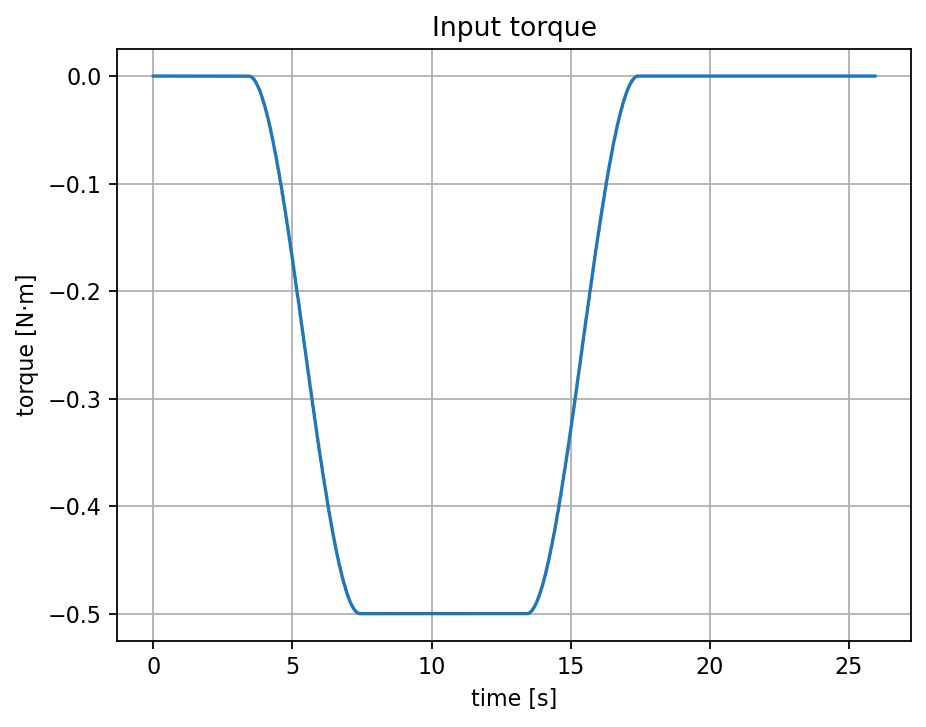
\includegraphics[scale=0.5]{images/chapter3/01_torque_vs_time.png}
    \caption{Input Torque Profile}
    \label{fig:01_torque_vs_time}
\end{figure}
\FloatBarrier

The smooth transitions between the zero and plateau levels are intentional: abrupt torque steps would excite the high-frequency modes of the numerical integrator and could temporarily drive the kinematic closure solver out of its convergence basin, particularly near the initial configuration where the warm-start has not yet built up a reliable history. The ramp duration of approximately two seconds provides a comfortable margin with respect to the integration step while keeping the overall experiment within a manageable time window.


\subsection{Reduced-Coordinate Kinematics}
The resulting evolution of the reduced coordinate $\theta$ is reported in Fig. \ref{fig:07_theta_kinematics}. Starting from the neutral position $\theta = 0rad$, the crank angle decreases monotonically during the torque ramp phase, reaching a minimum of approximately $-0.65 rad$ at $t \approx 10s$, which corresponds to the peak of the torque plateau. After the torque is removed, the passive elastic restoring forces encoded in the Fung exponential model of the finger joints partially recover the position, and $\theta$ settles at a steady-state value of approximately $-0.60rad$.

During the rising phase ($\tau_m = -0.5Nm \rightarrow 0Nm $) of the input torque, the crank angle exhibits an almost negligible variation, remaining close to its plateau value. This behavior indicates that the motor torque is primarily spent in overcoming static friction, the passive resistive torque of the finger, and the inertia of the mechanism, rather than producing motion. Only after these effects are compensated does the system start to evolve more significantly.

\begin{figure}[ht]
    \centering
    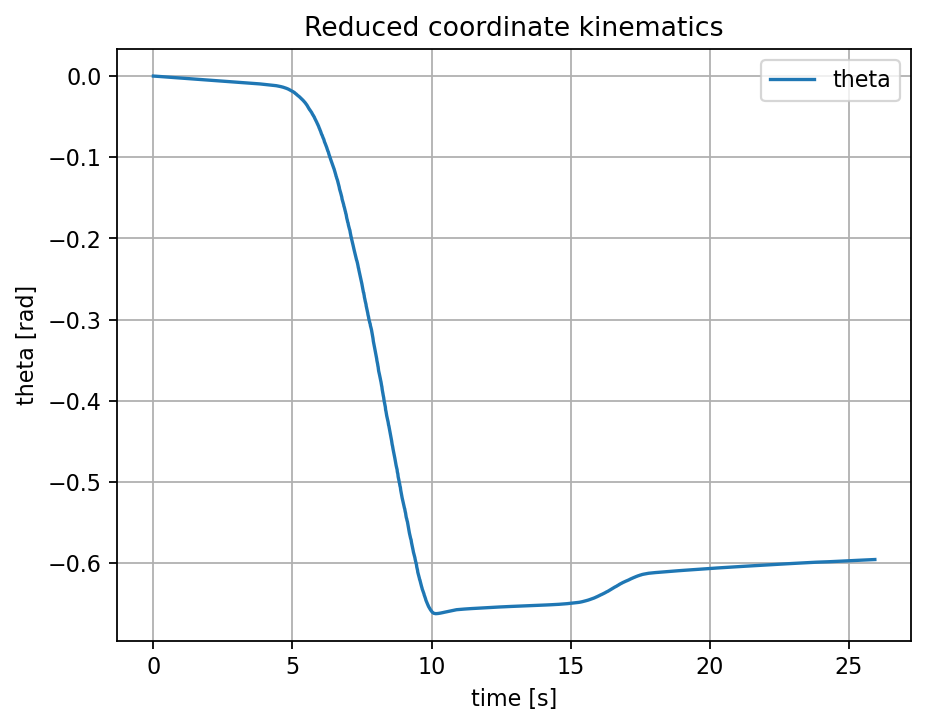
\includegraphics[scale=0.5]{images/chapter3/07_theta_kinematics.png}
    \caption{Reduced-Coordinate Kinematics}
    \label{fig:07_theta_kinematics}
\end{figure}
\FloatBarrier

Overall, the trajectory of $\theta$ exhibits the expected qualitative behaviour for a first-order dominated system with significant damping: the velocity is maximum during the steepest segment of the torque ramp (approximately $-0.9rad/s$ at $t \approx 8s$) and decays to near zero well before the torque plateau ends, indicating that the equilibrium between the applied torque, the growing passive restoring torque, and the viscous dissipation is reached before the torque is withdrawn. No oscillatory behaviour is observed, which is consistent with the overdamped nature of the chosen friction and passive stiffness parameters.

\subsection{Force at the CE Contact Point}
The magnitude of the force vector at the CE end-effector frame, estimated via the pseudo-inverse Jacobian method is plotted as a function of time in Fig. \ref{fig:02_ce_force_vs_time}. At the initial neutral configuration, a baseline force of approximately $0.14N$ is already present, which is entirely attributable to the gravitational loading of the distal links projected through the kinematic chain onto the contact frame. As the crank rotates in the negative direction and the finger mechanism flexes, the CE force rises monotonically, reaching a peak of approximately $0.30N$ at $t \approx 10s$.

After the torque is removed at $t \approx 18s$, the CE force does not return to its initial value but stabilises at approximately $0.28N$. This is consistent with the observed kinematics of $\theta$, which settles at a slightly flexed position due to the balance between the passive elastic restoring forces and the residual friction. The overall trend of the CE force closely follows the evolution of the crank angle, confirming that the reduced dynamic model correctly captures the relationship between the motor input, the passive finger mechanics, and the resulting end-effector interaction forces.

\begin{figure}[ht]
    \centering
    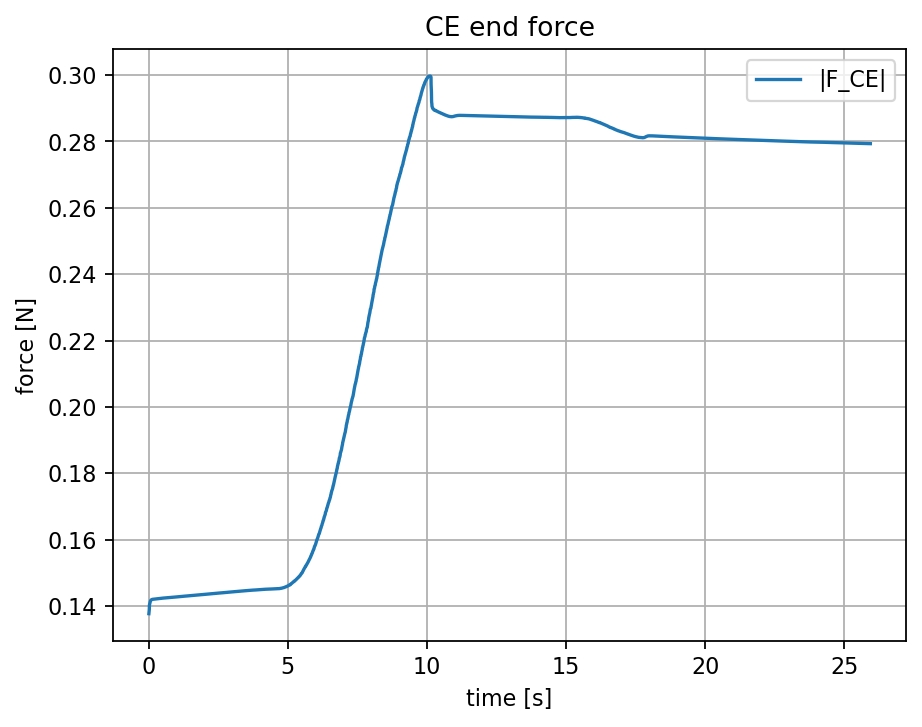
\includegraphics[scale=0.5]{images/chapter3/02_ce_force_vs_time.png}
    \caption{Force at the CE Contact Point}
    \label{fig:02_ce_force_vs_time}
\end{figure}
\FloatBarrier

\begin{figure}[ht]
    \centering
    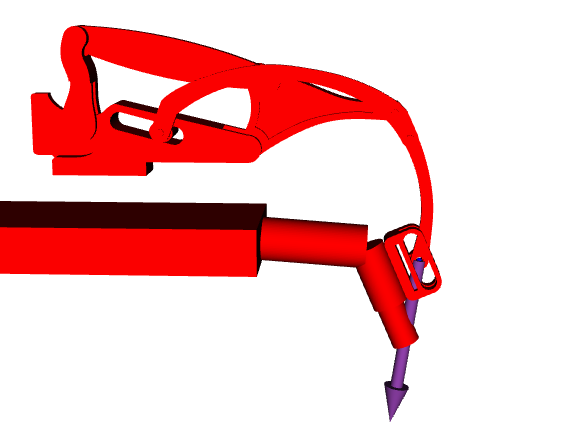
\includegraphics[scale=0.5]{images/chapter3/forza_end_effector.png}
    \caption{Force at the CE Contact Point}
    \label{fig:forza_end_effector}
\end{figure}
\FloatBarrier


\subsection{Kinematic Closure Solver Performance}
Figures \ref{fig:04_closure_norm} and \ref{fig:05_solver_diagnostics} report the numerical diagnostics of the kinematic closure solver over the course of the experiment.

\begin{figure}[ht]
    \centering
    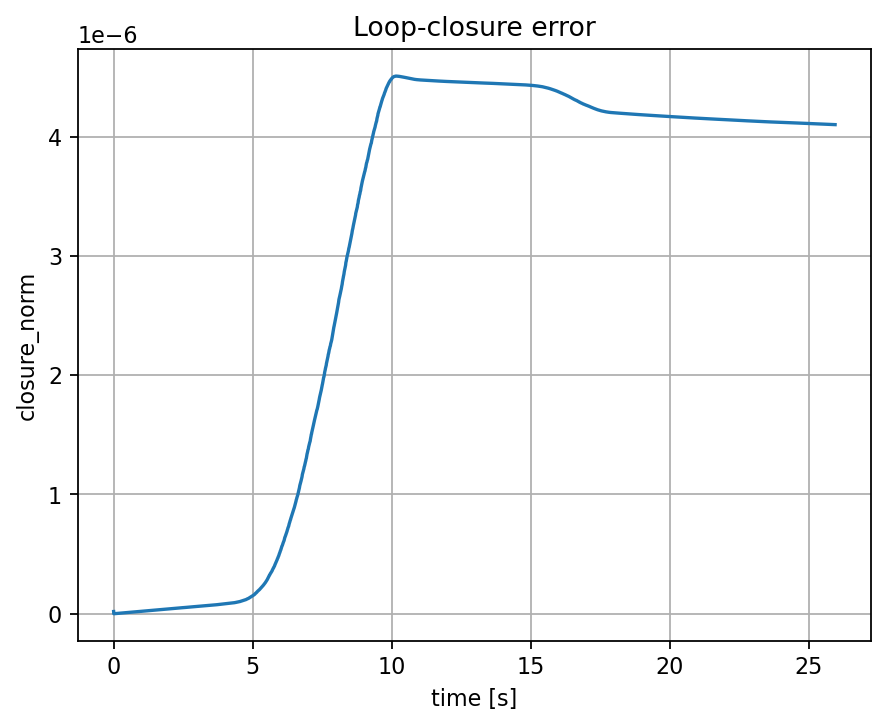
\includegraphics[scale=0.45]{images/chapter3/04_closure_norm.png}
    \caption{Norm of the Closure Error}
    \label{fig:04_closure_norm}
\end{figure}
\FloatBarrier

The closure residual norm $\|\mathbf{e}_\text{closure}\|$, defined as the Euclidean norm of the position mismatch across all four frame pairs, remains below $5 \times 10^{-6}m$ throughout the entire simulation. This value is well within the configured solver tolerance of $1 \times 10^{-5}m$, and corresponds to sub-micrometer errors at the physical scale of the mechanism (link lengths on the order of tens of millimetres). The residual increases during the dynamic phase of the simulation and then stabilises at a slightly higher plateau value of approximately $4.2 \times 10^{-6}m$. This mild increase is expected: as $\theta$ moves away from the neutral configuration, the nonlinearity of the constraint manifold becomes more pronounced, and the Trust Region Reflective (TRF) solver requires more iterations to converge to the same absolute accuracy. Nevertheless, the residual remains well bounded throughout, demonstrating the robustness of the warm-start strategy. 

\begin{figure}[ht]
    \centering
    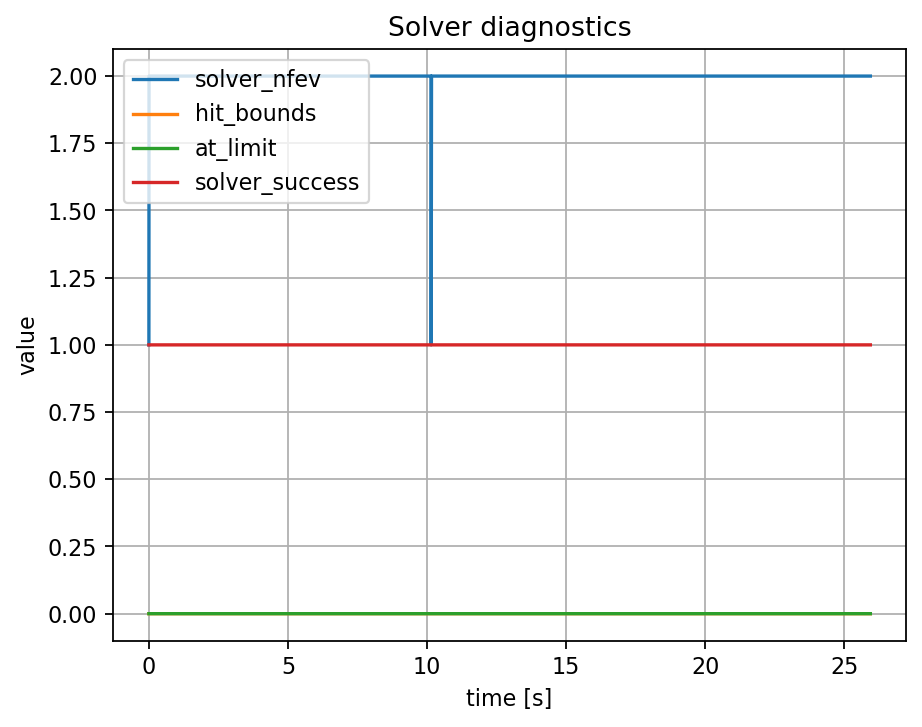
\includegraphics[scale=0.45]{images/chapter3/05_solver_diagnostics.png}
    \caption{Solver Diagnostics}
    \label{fig:05_solver_diagnostics}
\end{figure}
\FloatBarrier

The solver diagnostics panel (Fig. \ref{fig:05_solver_diagnostics}) confirms the efficiency of the warm-start mechanism. After a brief initialisation phase, the TRF solver consistently converges within only two function evaluations per step throughout the entire experiment. The convergence flag (\textit{solver\_success}) remains at unity (true) at all times, the \textit{hit\_bounds} flag never activates, indicating that none of the dependent joint variables reaches its prescribed bound, and the \textit{at\_limit} state machine flag remains at zero, confirming that the mechanism never enters the end-stop hold condition.

These results validate the real-time suitability of the closure algorithm: at a control frequency of 1 kHz, two function evaluations per step impose a computational overhead that is entirely compatible with the available hardware budget.


\subsection{Torque Breakdown on the Reduced Coordinate}
Figure \ref{fig:06_tau_breakdown} decomposes the total generalised torque acting on the reduced coordinate $\theta$ into its constituent contributions: the motor input $\tau_m$, the projected passive torque $\tau_{pass,\theta}$ and the friction torque $\tau_{fric}$.

\begin{figure}[ht]
    \centering
    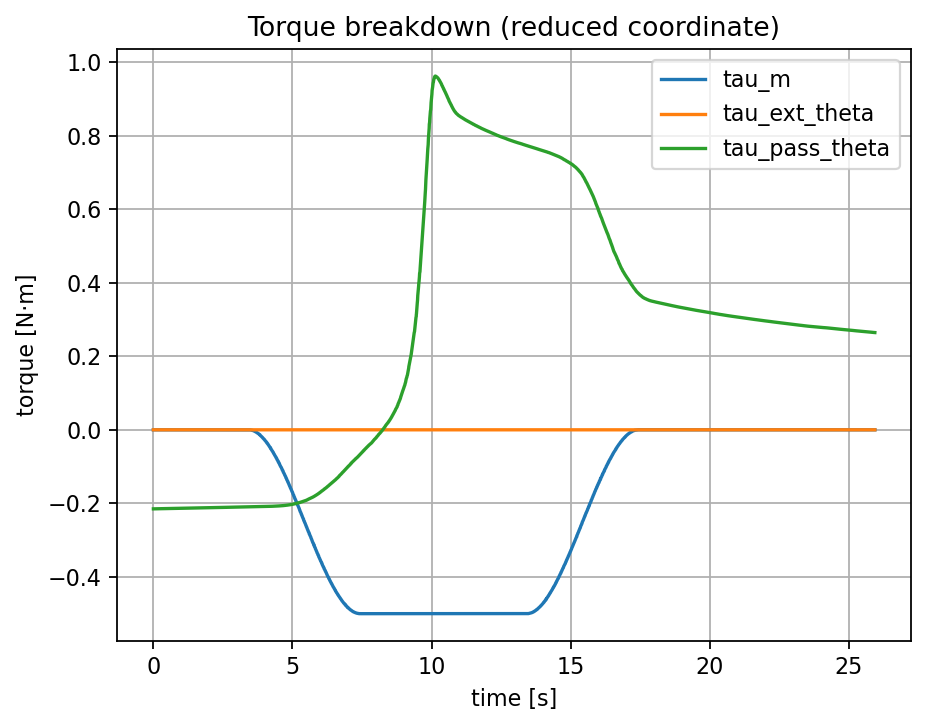
\includegraphics[scale=0.5]{images/chapter3/06_tau_breakdown.png}
    \caption{Torque Breakdown on the Reduced Coordinate}
    \label{fig:06_tau_breakdown}
\end{figure}
\FloatBarrier

As expected $\tau_{ext,\theta}$ remains identically zero throughout the experiment, since the external wrench publisher is disabled. The passive torque $\tau_{pass,\theta}$ evolves in a manner that is qualitatively consistent with the Fung exponential stiffness model: grows in magnitude as the mechanism flexes and the phalangeal joints depart further from their equilibrium positions, reaching a peak of approximately $1Nm$, and then decays as the mechanism partially recovers after the torque is removed. The sign convention is such that a positive opposes the flexion produced by the negative motor torque, consistent with the restoring role of the passive elastic elements.

The interaction between $\tau_m$ and $\tau_{pass,\theta}$ is particularly instructive. During the loading phase (approximately $t \in [4, 10]$), the motor torque drives $\theta$ in the negative direction while the passive torque grows in the opposing positive direction. The equilibrium is reached when the sum of the two contributions, minus the dissipative terms, approaches zero — which corresponds precisely to the point where $\dot{\theta} \rightarrow 0$ under constant applied torque, as observed in Fig. \ref{fig:07_theta_kinematics}. After the motor torque is withdrawn, the passive torque alone drives the mechanism back toward a partial recovery, settling at a new equilibrium dictated by the balance between the elastic restoring force and the Coulomb friction at the crank joint. This behaviour demonstrates that the Fung passive model, as implemented in \textit{compute\_passive\_torques()}, produces physically consistent dynamics and correctly captures the role of the finger tendons and capsular ligaments in limiting the range of motion and ensuring a passive return force on the actuated degree of freedom. 
 
\subsection{Summary}
The open-loop experiment presented in this section provides strong numerical and qualitative evidence for the correctness and robustness of the plant simulation prior to closing the control loop. The key findings are summarised as follows.

The kinematic closure solver maintains sub-tolerance residuals throughout a 26-second simulation involving significant crank displacements, converging in as few as two function evaluations per step thanks to the warm-start strategy. No limit-hold events or joint bound saturations are recorded, indicating that the chosen workspace lies well within the feasible region of the mechanism. The reduced-coordinate dynamics correctly captures the dominant physics of the system: the interplay between the motor torque, the passive finger stiffness, and the viscous and Coulomb dissipation produces kinematic trajectories that are qualitatively consistent with the expected behaviour of an overdamped single-degree-of-freedom system. Finally, the torque breakdown on the reduced coordinate confirms that the projected passive torque $\tau_{pass,\theta}$ dominates the dynamics at large crank displacements, a result that has direct implications for the design of the feedforward compensation term in the trajectory controller, as discussed in Chapter 4.
